Consider the eigenvalus BVP

$$u''(x)=\lambda u(x),\;\;\;u(0)=u(1)=0$$

which has eigenvalues $\lambda_n=-(n\pi)^2,\;n\in\mathbb{Z}^+$\\
a. Using finite differences, devise a numerical algorithm for computing these eigenvalues. Implement it
in Matlab and discuss how good the approximation is in terms of the mesh size $h$. Plot the
eigenfunctions for the first few eigenvalues.\\
b. Adapt your algorithm and code from a. to the eigenvalue BVP
$$u''(x)=\lambda u(x),\;\;\;u(0)=0,\;\;\;u'(1)+u(1)=0$$
for which the eigenvalues cannot be computed explicitly. Again, plot the first few eigenfunctions.\\
c. Consider the eigenvalue problem for the 2-dim Laplacian
$$\Delta u=\lambda u$$
in the unit square $[0,1]\times[0,1]$ with Dirichlett boundry conditions using the 5-point Laplacian and
explain how well the eigenvalues $\lambda_{m,n}=-(m^2+n^2)\pi^2$ are approximated. Plot eigenfunctions
for the first few eigenvalues.\\

\begin{solution}\renewcommand{\qedsymbol}{}\ \\
    a. We use the finite difference formula

    $$u''\approx\frac{U^{n+1}-2U^n+U^{n-1}}{h^2}=\lambda U^n$$

    Hence,

    $$U^{n+1}-(2+h^2\lambda)U^n+U^{n-1}=0$$

    This translates into the matrix equation

    $$\left(\begin{array}{ccccc} -2-h^2\lambda & 1 & 0 & \cdots & 0
                              \\ 1 & -2-h^2\lambda & \ddots & \ddots & \vdots \\ 0 & 1 & \ddots & 1 & 0
                              \\ \vdots & \ddots & \ddots & -2-h^2\lambda & 1
                              \\ 0 & \cdots & 0 & 1 & -2-h^2\lambda\end{array}\right)U=0$$
    
    That is

    $$(\left(\begin{array}{ccccc} -2 & 1 & 0 & \cdots & 0 \\ 1 & -2 & \ddots & \ddots & \vdots
                                \\ 0 & 1 & \ddots & 1 & 0 \\ \vdots & \ddots & \ddots & -2 & 1
                                \\ 0 & \cdots & 0 & 1 & -2 \end{array}\right)-h^2\lambda I)U$$
    $$=(A-h^2\lambda I)U=0$$
    
    So, we have the eigenvalue problem

    $$e_i=h^2\lambda$$

    This gives us an apporximation to the true eigenvalues with $\frac{e_i}{h^2}$ where $e_i$ is the
    $i^{th}$ eigenvalue of $A$. Since $h=\frac{1}{n+1}$ where $n$ is the number of steps in our
    interval, as $n$ gets larger, $h$ gets smaller, and so our approximation approaches the true
    eigenvalues with a smaller mesh size. This can be seen by changing the value for $n$ in the code
    seen below. This being solved before, we have that the general solutions for this particular BVP
    are $u(x)=\sin(\sqrt{-\lambda}x)$. For the first 3 eigenvalues, we have the following eigenfunctions
    plotted on the interval $[0,1]$.
    
    \begin{center}
        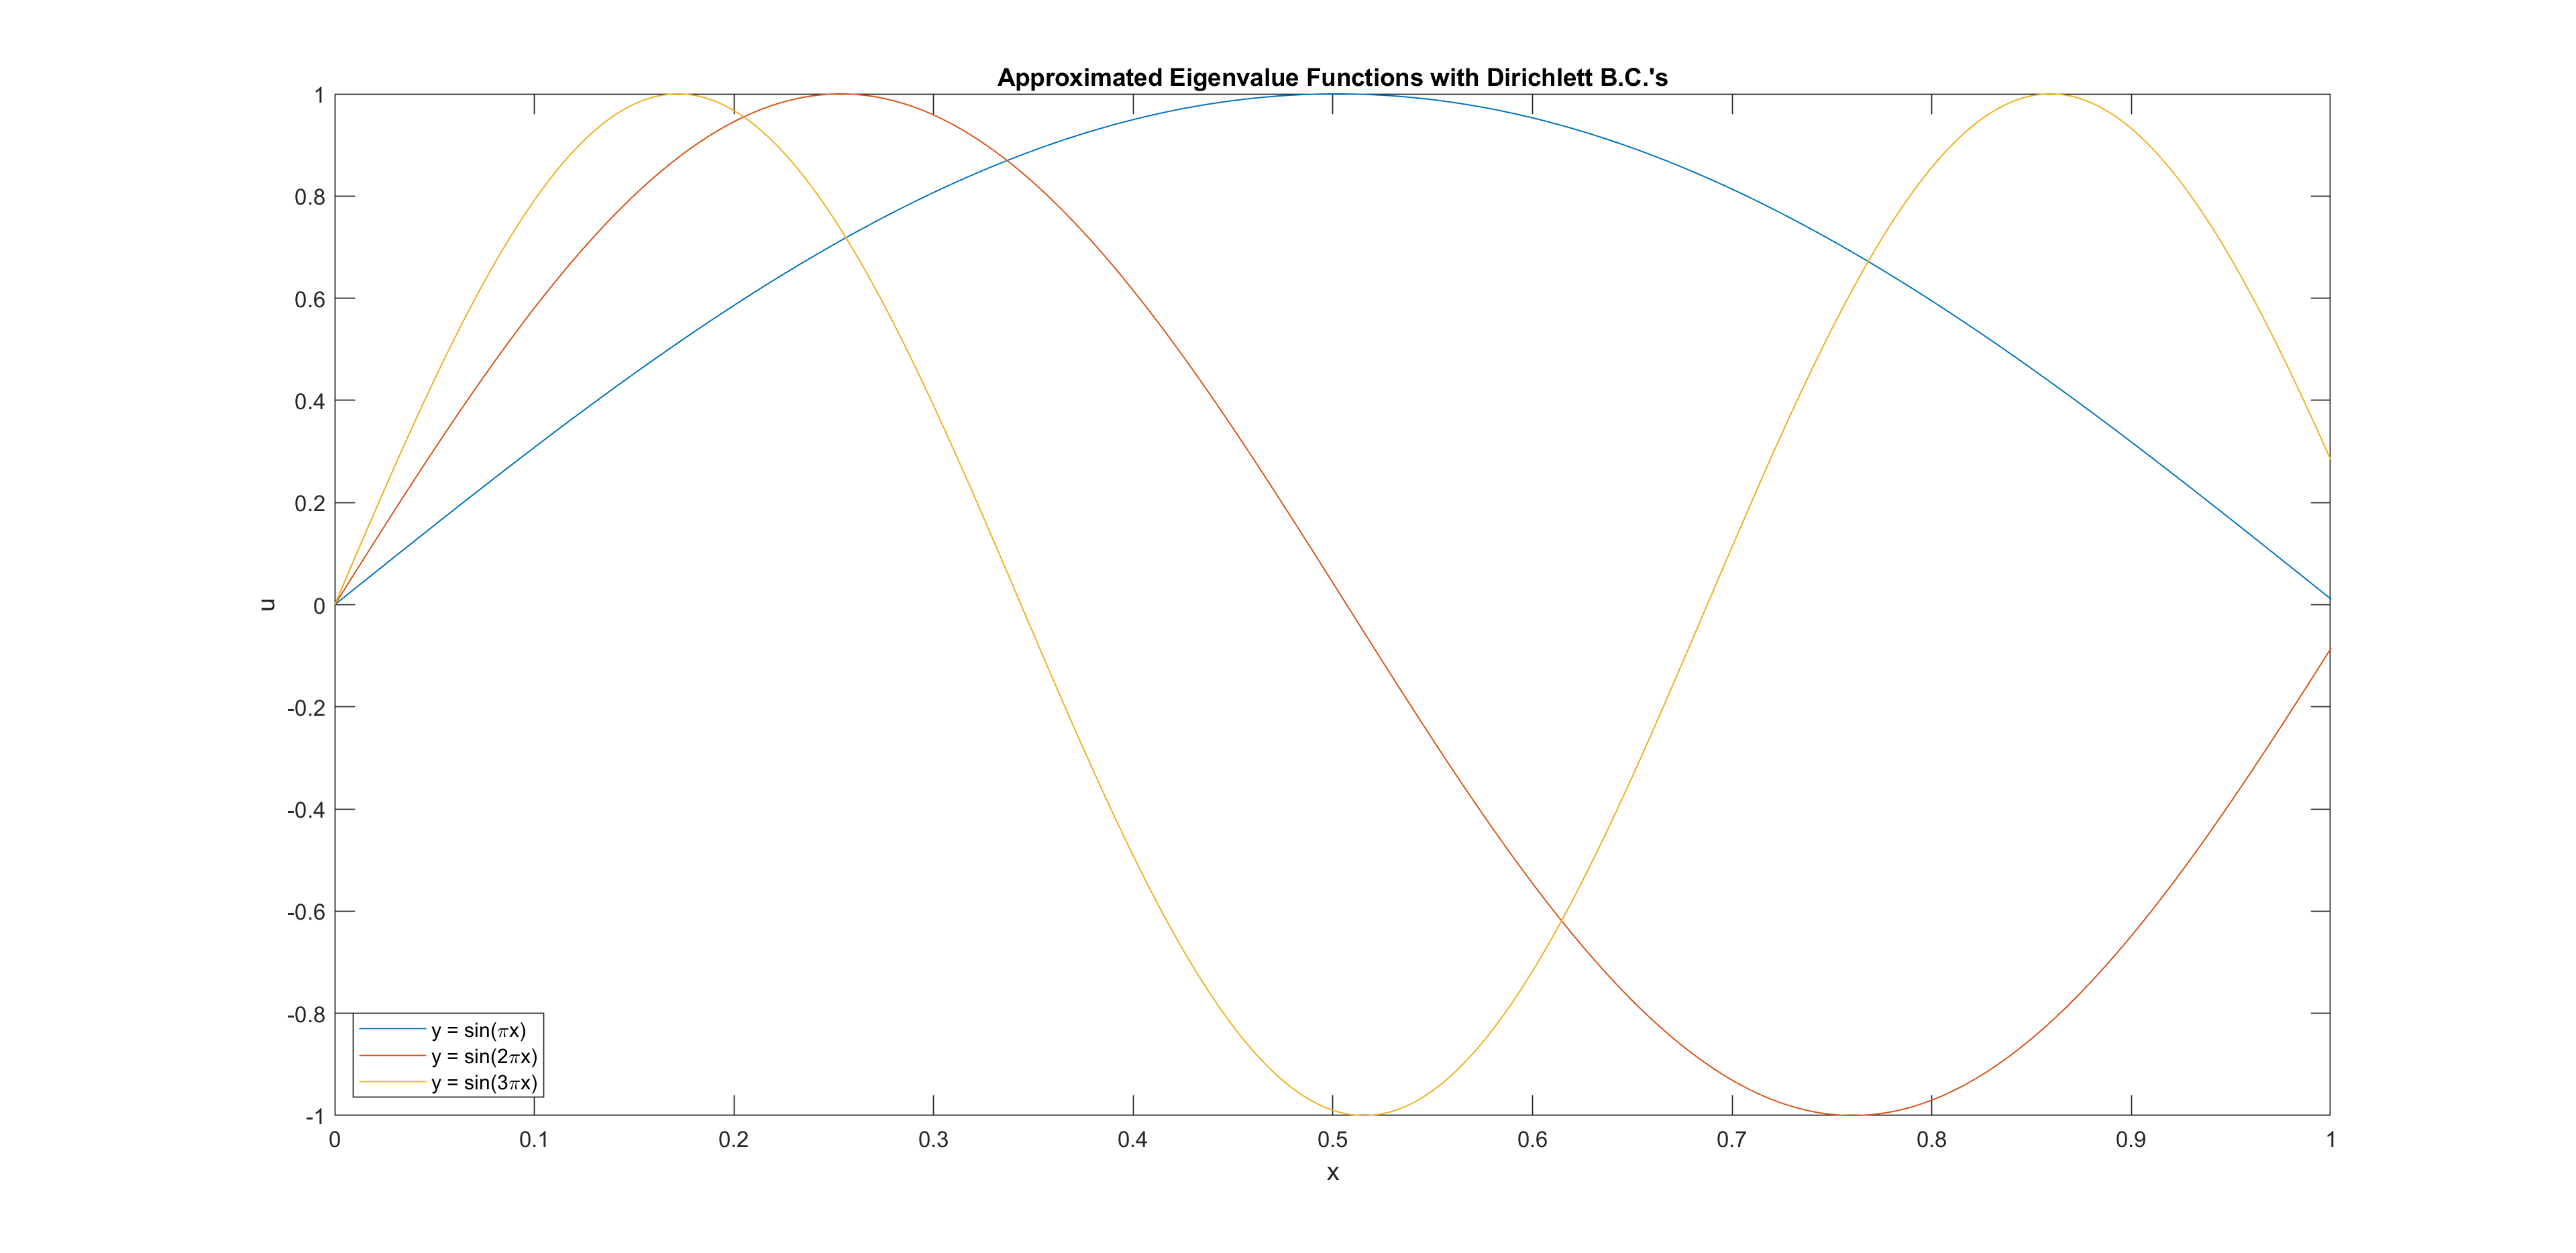
\includegraphics[scale=0.15]{1a.PNG}
    \end{center}

    b. We see that this problem will have similar general solutions, just with different eigenvalues to
    satisfy the new boundry condition $u'(1)+u(1)=0$. So, the adapted code utilizing the matrix equation

    $$AU=\lambda BU$$
    $$B=\left(\begin{array}{ccccc} 1 & 0 & 0 & \cdots & 0 \\ 0 & 1 & \ddots & \ddots & \vdots
                                \\ 0 & 0 & \ddots & 0 & 0\\ \vdots & \ddots & \ddots & 1 & 0
                                \\ 0 & \cdots & 0 & 0 & 0
        \end{array}\right)$$
    
    to find the eigenvalues of both $A$ and $B$ gives us the following 3 eigenfunctions, with the code
    below. Again, we also see that as the discretization increases, and our mesh size decreases. This
    yeilds better and better approximations and can be seen by chaging the values for $n$ in the code
    below.
    
    \begin{center}
        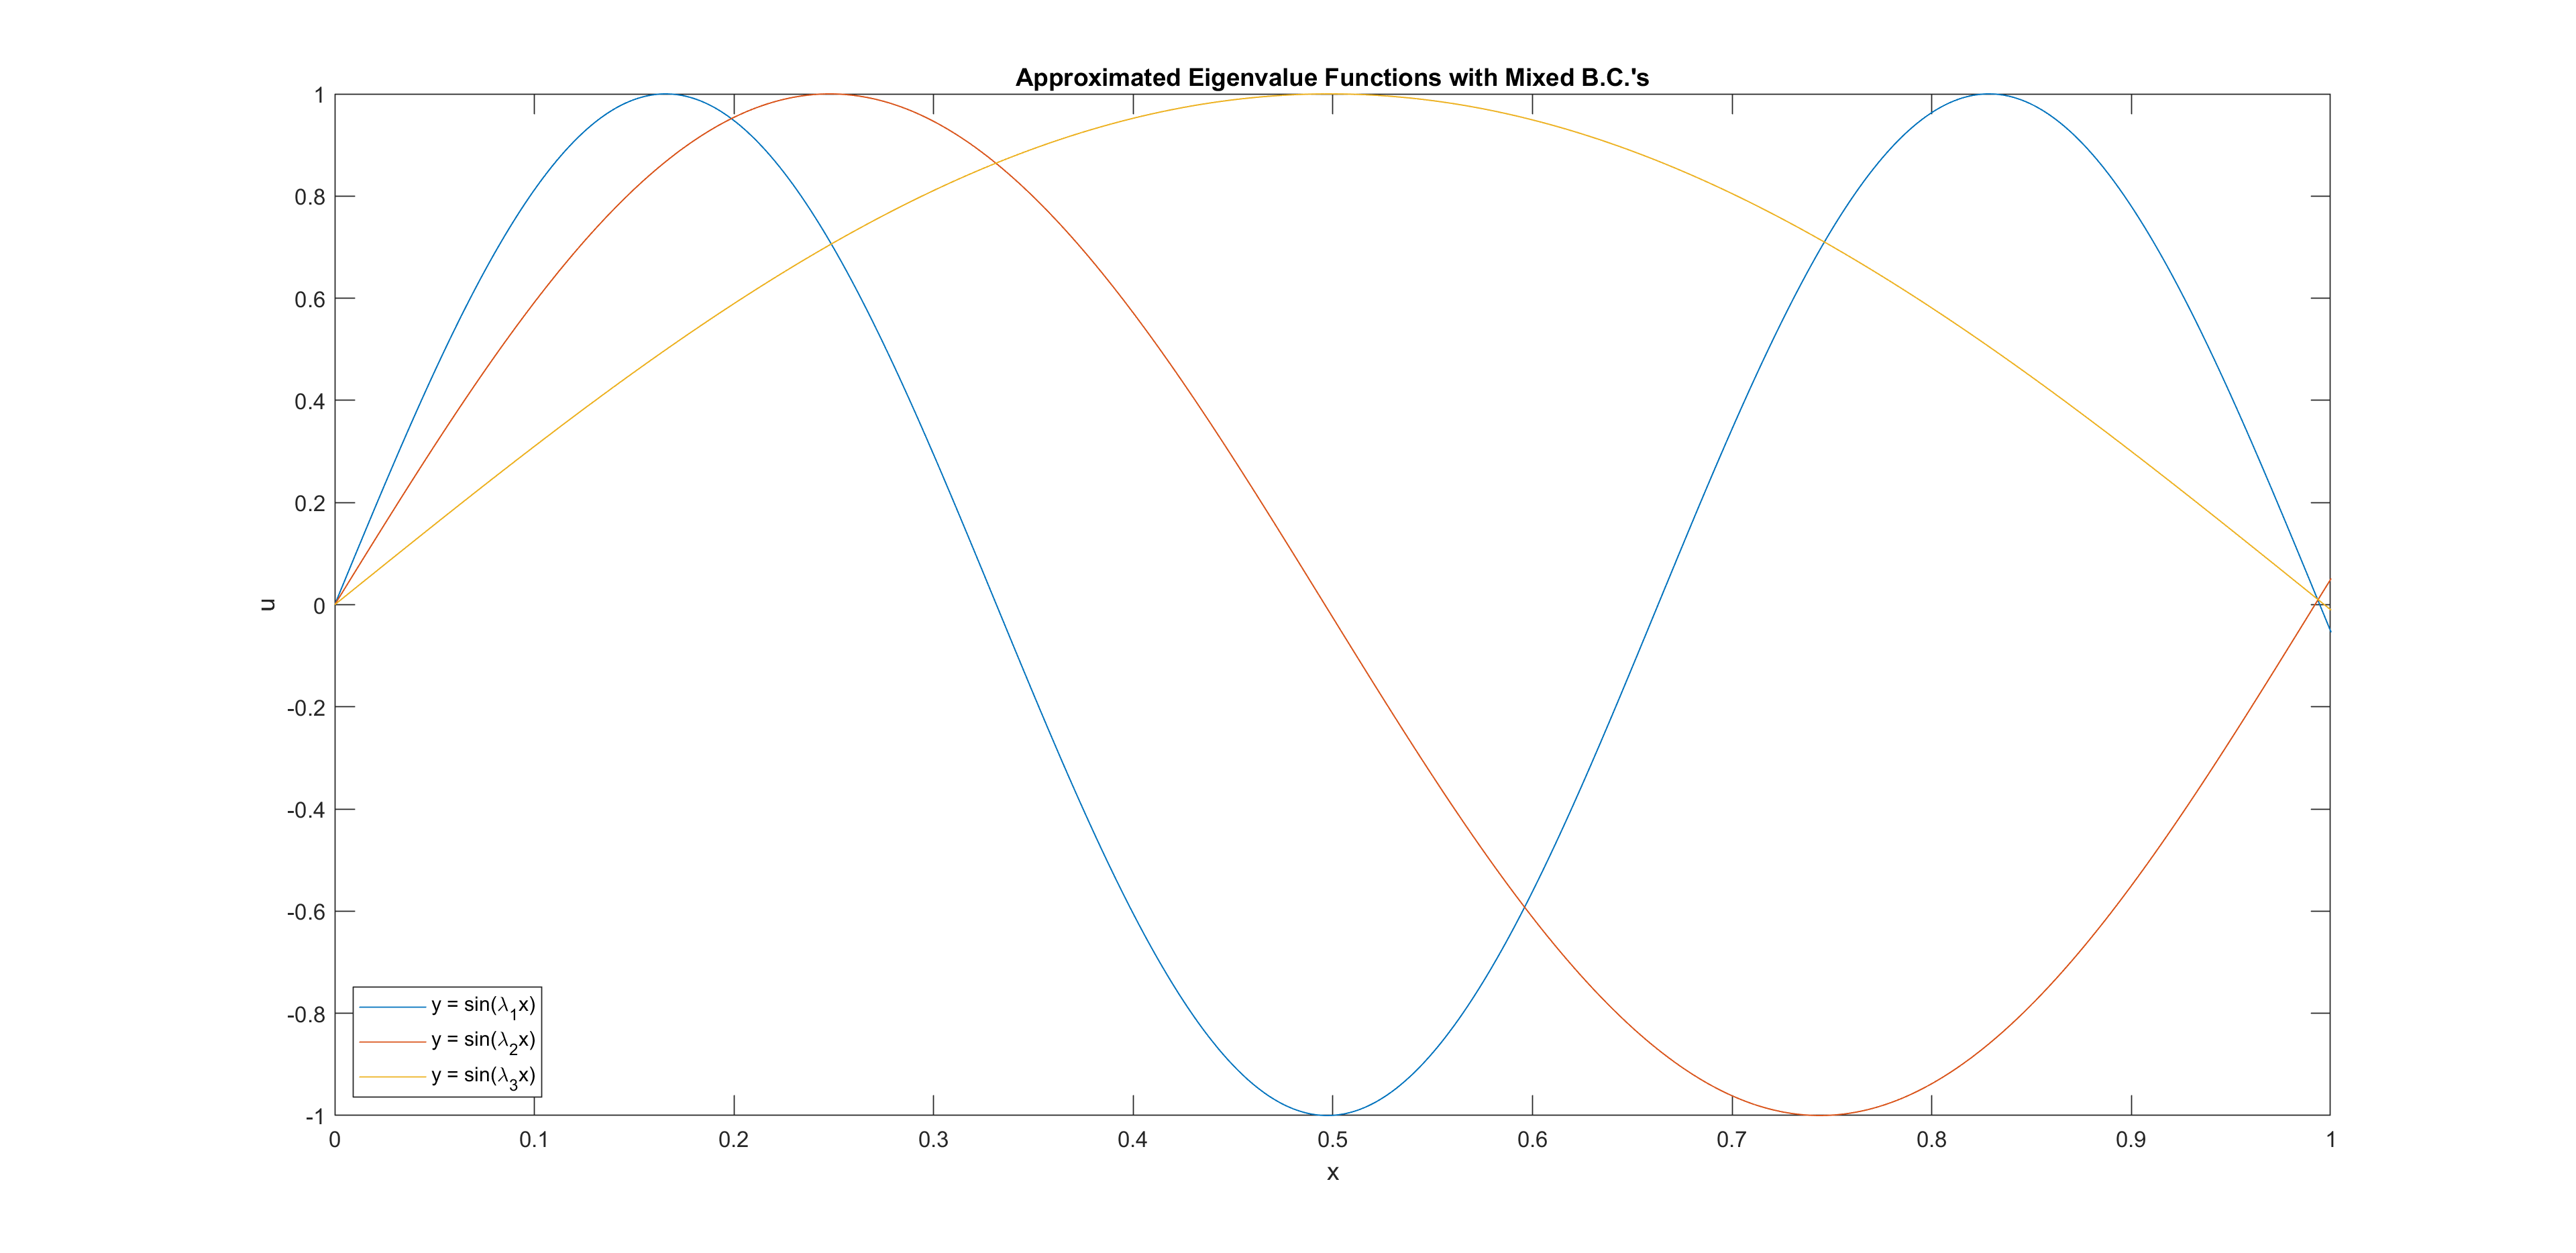
\includegraphics[scale=0.15]{1b.PNG}
    \end{center}

    c. For the closed unit square Laplace equation with Dirichlett boundry conditions, we utilized the
    code from the 5-point Laplacian. For this approximation, we made the distinction between the
    discretization on $x$ and on $y$. This allows us to find more distinct eigenvalues and also see how
    having unequal mesh sizes impairs the approximations. So, for this, we used $m=n$ so that the
    approximations were closer, and as in the previous two questions, we have that the larger $m,n$, the
    better the approximations become. The values for $m$ and $n$ can be changed in the code below.
    
    \begin{center}
        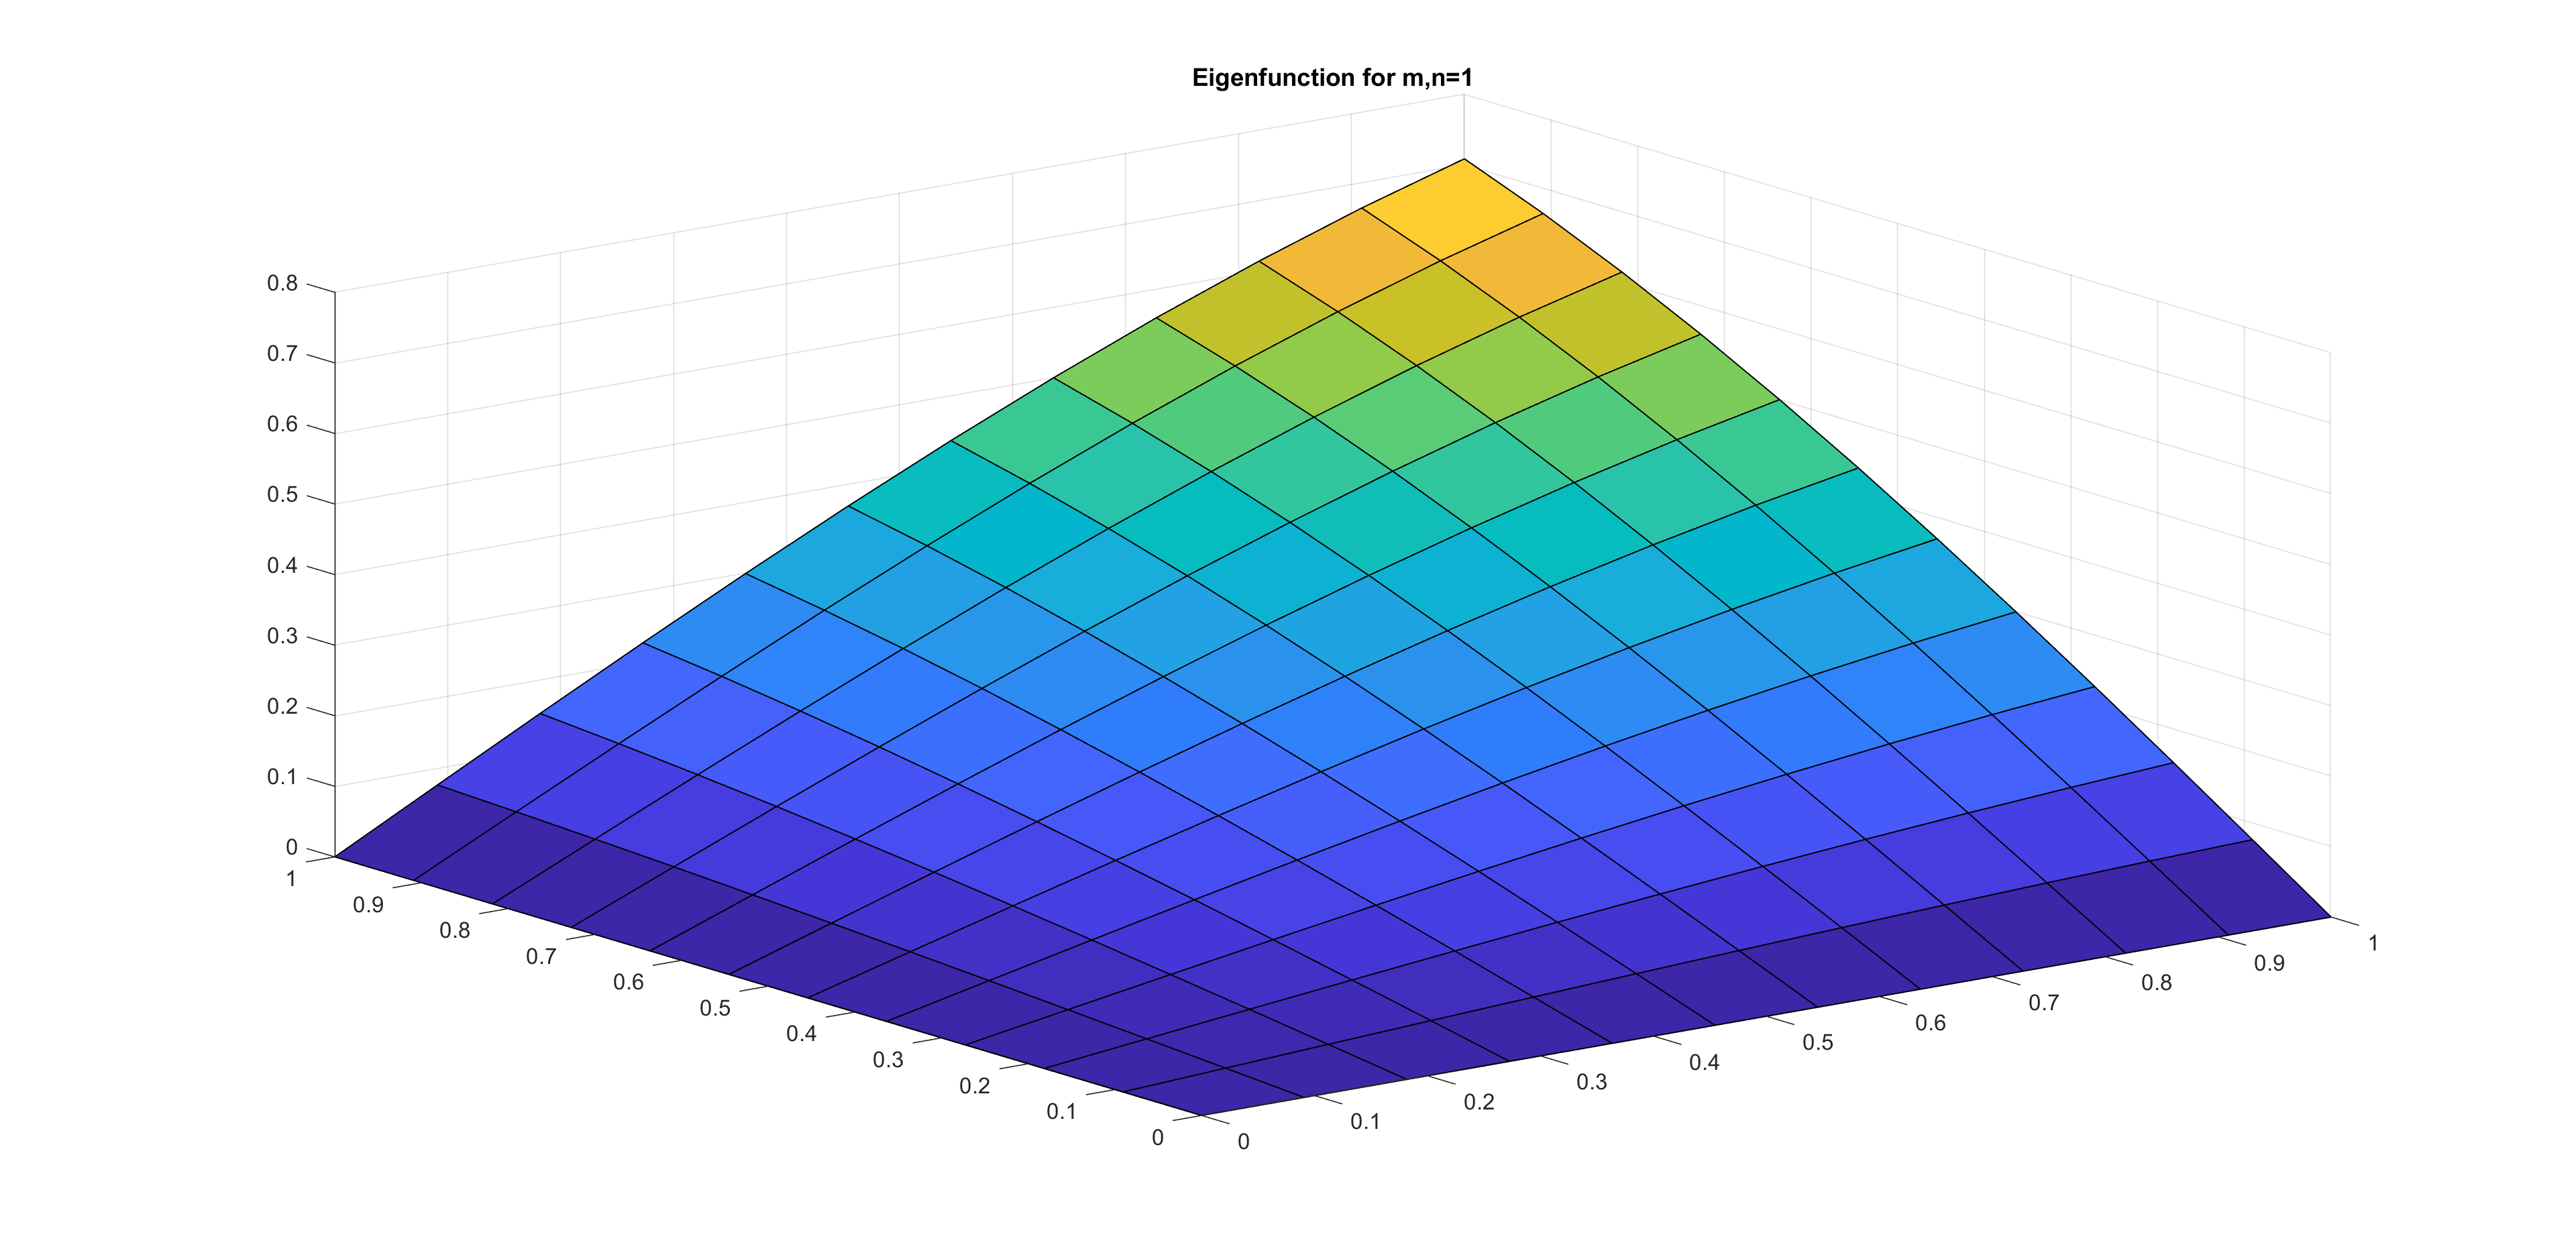
\includegraphics[scale=0.15]{1c11.PNG}
    \end{center}
    \begin{center}
        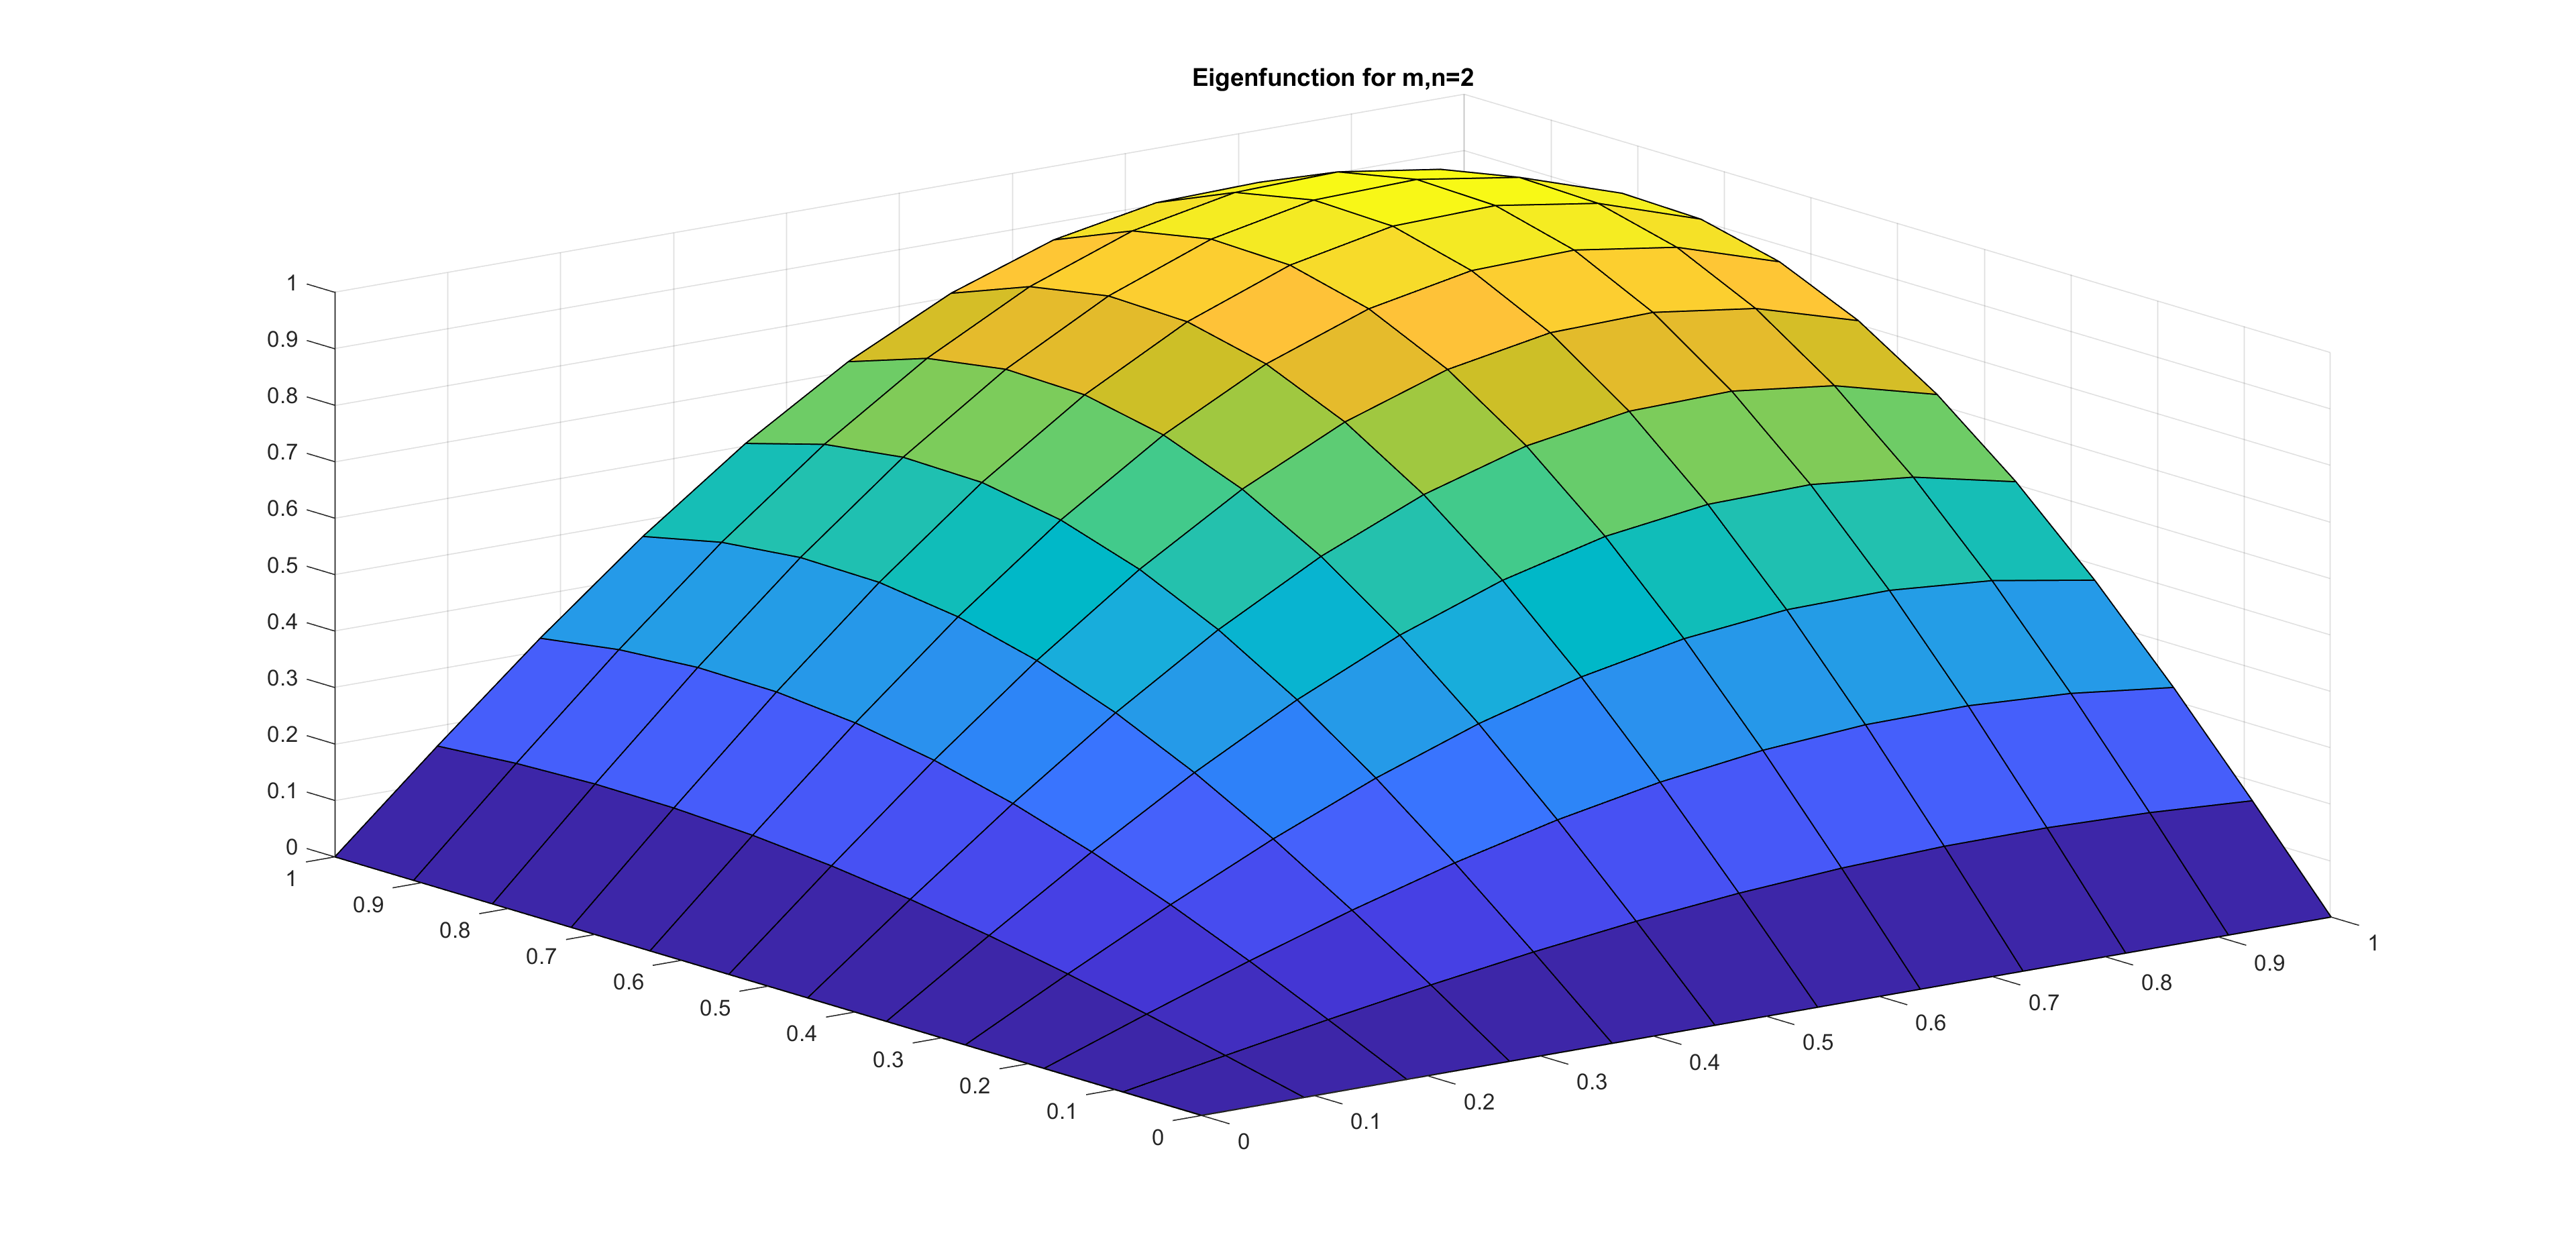
\includegraphics[scale=0.15]{1c22.PNG}
    \end{center}
    \begin{center}
        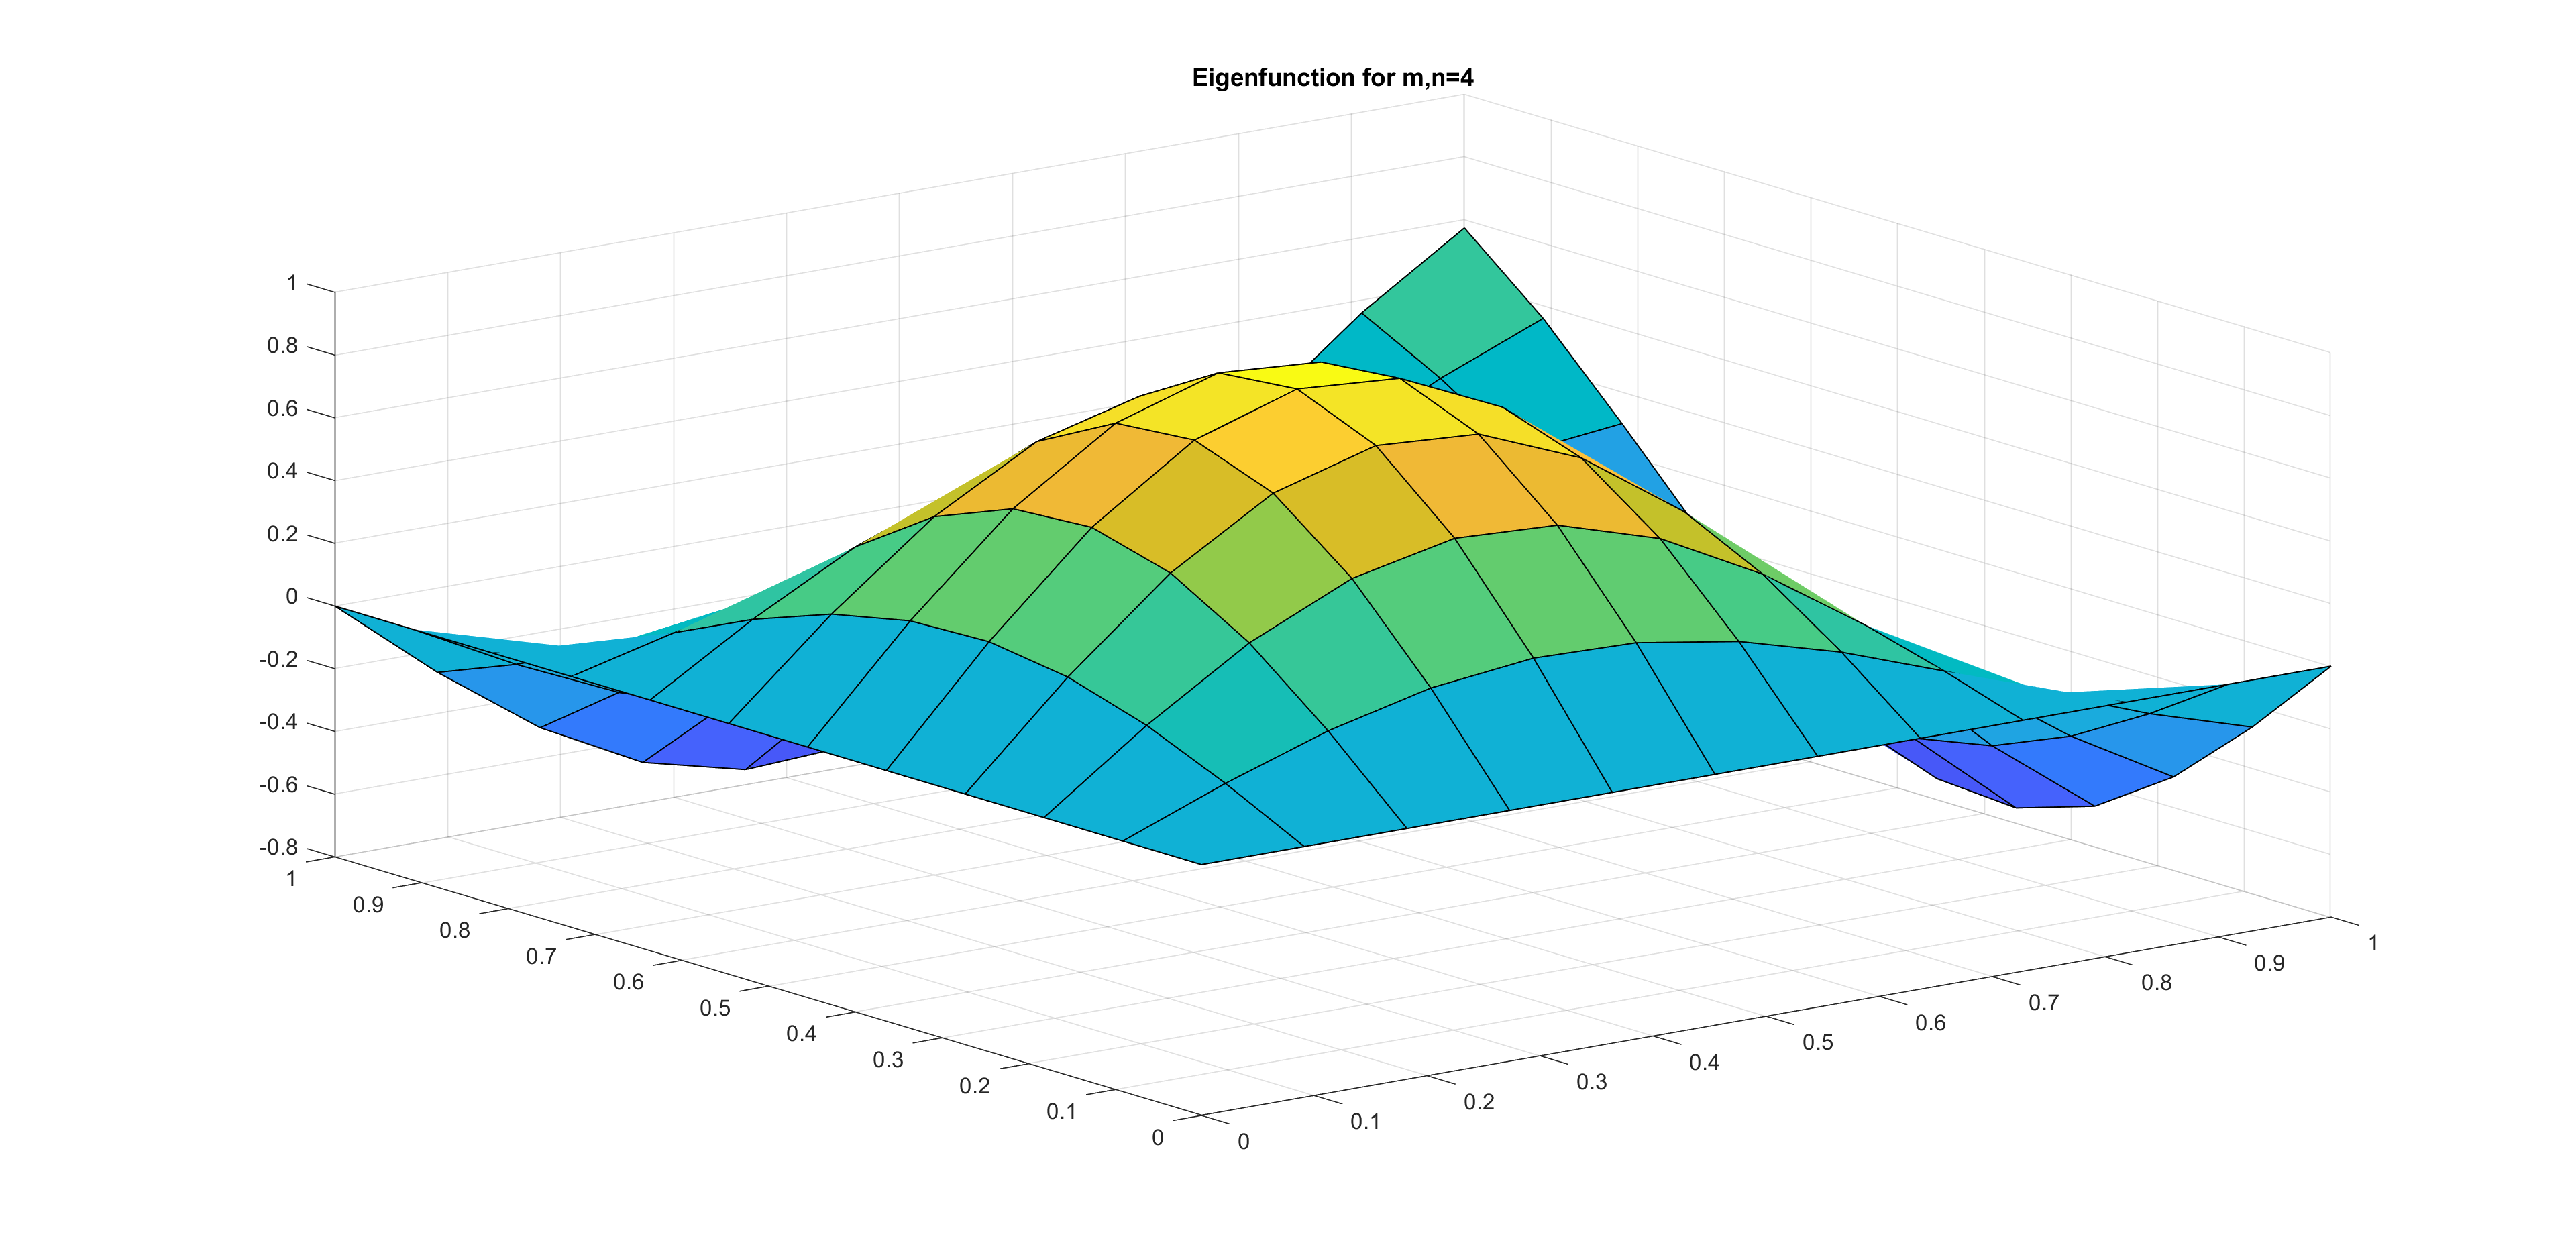
\includegraphics[scale=0.15]{1c44.PNG}
    \end{center}

\end{solution}

\newpage
\lstinputlisting{num1a.m}
\newpage
\lstinputlisting{num1b.m}
\newpage
\lstinputlisting{num1c.m}